\documentclass[11pt,a4paper]{article}

% --- Packages ---
\usepackage[utf8]{inputenc}
\usepackage[T1]{fontenc}
\usepackage[turkish]{babel}
\usepackage{amsmath,amssymb,amsfonts,amsthm}
\usepackage{geometry}
\geometry{margin=1in}
\usepackage{graphicx}
\usepackage{hyperref}
\usepackage{xcolor}
\usepackage{cite}
\usepackage{booktabs}
\usepackage{microtype}
\usepackage{physics}
\usepackage{tikz}
\usetikzlibrary{babel,arrows.meta}
\usepackage{listings}

\hypersetup{
    pdftitle={Büzülen Atom Metriği ve Konformal Eylem İlkesi: Karanlık Enerjisiz Bir Evrende Tip Ia Süpernova (Pantheon+) ve Kozmolojik Testler},
    pdfauthor={Muhammed Furkan Haydari},
    pdfsubject={Kozmoloji, Tip Ia Süpernova, Pantheon+, Büzülen Atom Metriği},
    pdfkeywords={Konformal Kozmoloji, Pantheon+, Tolman Testi, Etherington İkiliği, Hubble Gerilimi},
    colorlinks=true,
    linkcolor=blue!70!black,
    citecolor=red!70!black,
    urlcolor=blue!80!black
}

% --- Listings Settings ---
\definecolor{codegreen}{rgb}{0,0.55,0.2}
\definecolor{codegray}{rgb}{0.45,0.45,0.45}
\definecolor{codepurple}{rgb}{0.55,0.1,0.75}
\definecolor{codeblue}{rgb}{0.1,0.2,0.8}
\definecolor{backcolour}{rgb}{0.97,0.97,0.98}

\lstdefinestyle{pythoncode}{
    backgroundcolor=\color{backcolour},   
    commentstyle=\color{codegreen}\itshape,
    keywordstyle=\color{codeblue}\bfseries,
    numberstyle=\tiny\color{codegray},
    stringstyle=\color{codepurple},
    basicstyle=\ttfamily\scriptsize,
    breaklines=true,                 
    captionpos=b,                    
    numbers=left,                    
    numbersep=6pt,                  
    frame=single,
    rulecolor=\color{gray!30}
}
\lstset{style=pythoncode}

% --- Theorem Environments ---
\newtheorem{theorem}{Teorem}[section]
\newtheorem{definition}{Tanım}[section]
\newtheorem{axiom}{Aksiyom}[section]
\newtheorem{corollary}{Sonuç}[theorem]
\newtheorem{lemma}[theorem]{Lemma}
\newtheorem{remark}{Not}[section]

\title{\textbf{Büzülen Atom Metriği ve Konformal Eylem İlkesi: \\ Karanlık Enerjisiz Bir Evrende Tip Ia Süpernova (Pantheon+) ve Kozmolojik Testler}}

\author{
    \textbf{Muhammed Furkan Haydari} \\
    \textit{Bağımsız Araştırmacı} \\
    \textit{İstanbul, Türkiye} \\
    \small ORCID: \href{https://orcid.org/0009-0003-2854-3947}{0009-0003-2854-3947} \quad$\bullet$\quad \small DOI: \href{https://doi.org/10.5281/zenodo.23633034}{10.5281/zenodo.23633034}
}

\date{\today}

\begin{document}
\shorthandoff{=}

\maketitle

\begin{abstract}
    Standart $\Lambda$CDM kozmolojisi, kozmolojik kırmızıya kaymayı uzay-zamanın genişlemesi olarak yorumlamakta; ancak bu çerçeve kuramsal ve gözlemsel olarak karanlık enerji ince ayarı, kozmik şişme başlangıç koşulları ve Hubble gerilimi ($H_0$ tension) gibi önemli sorularla karşılaşmaktadır. Bu çalışmada, uzay-zaman metriğinin statik ve düz Minkowski sürekliliği ($\eta_{\mu\nu}$) olarak modellendiği, kozmolojik kırmızıya kaymanın ise yerel atomik uzunluk cetvellerinin konformal skalar alan dinamikleri uyarınca zaman içinde büzüşmesinden ($r_{\mathrm{atom}}(t) = r_0 (1+z)^{-1}$) kaynaklandığı bir konformal kozmoloji modeli incelenmektedir.

    Modelin dinamik temellerini konformal skalar-tensör eyleminden varyasyonel olarak inşa ediyoruz: $V(\chi) = -\frac{1}{2} H_0^2 \chi^2$ vakum potansiyeli altında skalar alanın hareket denklemi çözüldüğünde, evrensel ölçek büzülmesinin ($\dot{\lambda}/\lambda = -H_0$) kararlı bir kozmolojik atraktör olarak ortaya çıktığı gösterilmektedir. Fotonların sıfır (null) geodezikleri boyunca statik Öklid uzayında katettiği mesafe üzerinden, Parlaklık Mesafesi (Luminosity Distance) birinci ilkelerden analitik olarak $d_L(z) = \frac{c}{H_0} (1+z) \ln(1+z)$ biçiminde türetilmektedir. Hiçbir serbest karanlık enerji parametresi ($\Omega_\Lambda \equiv 0$) içermeyen bu tek serbest parametreli ($H_0$) model, resmi Pantheon+ Tip Ia Süpernova veri seti ve tam kovaryans matrisi ile test edilmiş; $H_0 = 70.75 \pm 0.14\text{ km/s/Mpc}$ değeriyle 26 binned veri üzerinde $\chi^2_{\mathrm{cov}}/\text{dof} = 3.748$, tam $N=1580$ binned olmayan Hubble akışı üzerinde ise $\chi^2_{\mathrm{cov}}/\text{dof} = 0.945$ elde edilerek karanlık enerji serbest parametresine gerek duymayan istatistiksel bir alternatif sunulmuştur.

    Ayrıca alternatif statik modellere yöneltilen iki kritik gözlemsel test analitik olarak ele alınmaktadır: (i) Konformal metrik dönüşümlerinde Etherington karşılıklılığı ($d_L = (1+z)^2 d_A$) korunduğundan, gözlemlenen yüzey parlaklığı Tolman $(1+z)^{-4}$ sönümleme kuralını tam olarak sağlar ve Lubin--Sandage testiyle uyum gösterir; (ii) Erken kozmolojik dönemde baryon-foton optik derinliğinin büyüklüğü ($\tau \gg 1$) ve $A=5, 8$ kararsızlık boğazı ile alfa vadisinin termodinamik dengesi, evrendeki \%25'lik ilksel Helyum-4 bolluğunu ve 2.73 K CMB kara cisim termalizasyonunu durağan bir temsilde anlamlandırmaya yönelik tutarlı bir çerçeve sunar.
\end{abstract}

\vspace{1em}
\noindent\textbf{Anahtar Kelimeler:} Konformal Kozmoloji, Büzülen Madde Metriği, Pantheon+ Süpernova, Karanlık Enerji, Tolman Yüzey Parlaklığı, Eylem İlkesi, Etherington İkiliği.

\vspace{1em}
\hrule
\vspace{0.8em}
\tableofcontents
\vspace{0.8em}
\hrule
\vspace{1.5em}

\section{Giriş ve Konformal Çerçevelerin Gözlemsel Motivasyonları}
\label{sec:giris_kozmo}

Modern gözlemsel kozmoloji, genişleyen Friedmann--Lema\^itre--Robertson--Walker (FLRW) metriğine dayanan standart $\Lambda\mathrm{CDM}$ modeli üzerine kuruludur. Bu model büyük ölçekli yapıların dağılımını ve Tip Ia süpernova gözlemlerini~\cite{riess1998,perlmutter1999} açıklamakta başarılı olmuşsa da, kuramsal ve gözlemsel olarak önemli sorular barındırmaktadır:
\begin{enumerate}
    \item \textbf{Kozmolojik Sabit Problemi:} Gözlemlenen karanlık enerji yoğunluğu ($\rho_\Lambda \sim 10^{-47}\text{ GeV}^4$), kuantum alan teorisindeki vakum sıfır noktası enerjisi kestirimlerinden çok daha küçüktür.
    \item \textbf{Hubble Gerilimi ($H_0$ Tension):} Erken evren (Planck CMB) ölçümleri ($H_0 \approx 67.4\text{ km/s/Mpc}$) ile yerel evren (SH0ES Tip Ia süpernova ve Cepheid) ölçümleri ($H_0 \approx 73.0\text{ km/s/Mpc}$) arasında $5\sigma$ düzeyinde istatistiksel bir uyuşmazlık mevcuttur.
    \item \textbf{JWST Erken Olgun Galaksileri:} James Webb Uzay Teleskobu'nun $z > 10$ bölgesinde keşfettiği yüksek kütleli, parlak ve metalliğe sahip olgun galaksiler, standart hiyerarşik yapı oluşumunun izin verdiği ilk 300 milyon yıllık zaman penceresi için zorlayıcı kısıtlar getirmektedir.
\end{enumerate}

Christof Wetterich~\cite{wetterich2013} ve Fred Hoyle~\cite{hoyle1964} tarafından vurgulandığı üzere, bir uzay-zaman manifoldunun genişlemesi ile o manifold içinde yaşayan parçacıkların yerel kütle ve uzunluk ölçeklerinin büzülmesi arasında tam bir \textbf{konformal denklik (conformal equivalence)} kurulabilir. Bu çalışmada, uzayın genişlemesi varsayımına alternatif olarak, arka planın statik düz Minkowski uzayı olarak modellendiği ve gözlemlenen kozmolojik dinamiklerin atomların konformal skalar alan gradyanı boyunca büzülmesinden kaynaklandığı odaklanmış bir kozmoloji çerçevesi incelenmektedir.

\section{Konformal Skalar-Tensör Eylemi ve Büzülme Alan Denklemleri}
\label{sec:eylem_ilkesi_kozmo}

Modelimizin dinamik temelini, yerel kütle ölçeğini belirleyen dinamik bir $\chi(x)$ skalar alanı üzerinden inşa ediyoruz. Parçacık kütleleri $m_i(\chi) = y_i \chi$ biçiminde Yukawa kuplajlarıyla bu alana bağlıdır; dolayısıyla atomik uzunluk cetvelleri $r_{\mathrm{atom}}(\chi) \propto \chi^{-1}$ ters orantısıyla belirlenir.

Toplam gravitasyonel ve skalar alan eylemi:
\begin{equation}
    S[\chi, g_{\mu\nu}] = \int d^4x \sqrt{-g} \left[ \frac{1}{2} \chi^2 R - \frac{1}{2} g^{\mu\nu} \partial_\mu \chi \partial_\nu \chi - V(\chi) + \mathcal{L}_{\mathrm{madde}}(g_{\mu\nu}, \psi, \chi) \right],
    \label{eq:konformal_eylem}
\end{equation}
olarak tanımlanır. Bu eylemin $\chi$ skalar alanına göre varyasyonu ($\delta S / \delta \chi = 0$), aşağıdaki hareket denklemini dikte eder:
\begin{equation}
    \Box \chi - \chi R + \frac{dV}{d\chi} = -\frac{\partial \mathcal{L}_{\mathrm{madde}}}{\partial \chi} = \frac{1}{\chi} T^\mu_{\mu(\mathrm{madde})}.
    \label{eq:chi_hareket}
\end{equation}

Birleşik Büzülme Hipotezi'nin temel aksiyomu uyarınca fiziksel arka plan uzay-zamanı Öklid sürekliliğidir; dolayısıyla metrik tensör düz Minkowski zeminidir ($g_{\mu\nu} = \eta_{\mu\nu} = \text{diag}(-c^2, 1, 1, 1)$, Ricci skaları $R \equiv 0$, $\sqrt{-g}=1$). Homojen kozmolojik ölçekte ($\nabla \chi = 0$) d'Alembertian operatörü $\Box \chi = -\frac{1}{c^2}\ddot{\chi}$ olur. Doğal birimlerde ($c=1$) skalar potansiyel:
\begin{equation}
    V(\chi) = -\frac{1}{2} H_0^2 \chi^2,
    \label{eq:potansiyel_secimi}
\end{equation}
olarak belirlendiğinde, serbest varyasyonel alan denklemi ($\ddot{\chi} - \frac{dV}{d\chi} = 0$):
\begin{equation}
    \ddot{\chi}(t) - H_0^2 \chi(t) = 0 \implies \chi(t) = c_1 e^{H_0 t} + c_2 e^{-H_0 t},
    \label{eq:chi_cozum}
\end{equation}
haline gelir. Pozitif yönde evrilen geç-zaman kozmolojik atraktör çözümü:
\begin{equation}
    \chi(t) = \chi_0 e^{H_0 t},
\end{equation}
biçiminde tekilleşir.

Atomik uzunluk standardını $\lambda(t) \equiv \chi_0 / \chi(t)$ olarak tanımladığımızda:
\begin{equation}
    \lambda(t) = e^{-H_0 t} \implies \frac{\dot{\lambda}(t)}{\lambda(t)} = -H_0.
    \label{eq:hubble_baryon}
\end{equation}
\textbf{Kuramsal Sonuç ve Ölçek Kalkülüsü:} Evrensel ölçek daralması temposu ($H_0$), düz Minkowski zemininde yaşayan konformal skalar alan teorisinin \textbf{kararlı bir kozmolojik atraktörüdür.} 

\subsection{Enerji-Momentum Korunumu ve Einstein Çerçevesi Denkliği (Weyl Ayar Değişmezliği)}
\label{sec:weyl_denkliği}

Burada haklı bir teorik itiraz akla gelebilir: \textit{``$\chi(t) = \chi_0 e^{H_0 t}$ skalar alanının basıncı ($p_\chi = H_0^2\chi^2$) sıfır değilse, uzay-zaman manifoldunun metriği ($\eta_{\mu\nu}$) bu basınca tepki vermeden (backreaction olmaksızın) nasıl mutlak düz kalabilir?''}

Bu açmaz, konformal skalar-tensör teorilerinde \textbf{Weyl Ayar Değişmezliği (Weyl Gauge Invariance)} ve çerçeve dönüşümü ile eksiksiz çözülür:
\begin{enumerate}
    \item Konformal eşlenim parametresi $\xi = 1/6$ seçildiğinde, skalar alanın Callan--Coleman--Jackiw (CCJ) iyileştirilmiş enerji-momentum tensörü:
    \begin{equation}
        \Theta_{\mu\nu} = \partial_\mu\chi\partial_\nu\chi - \frac{1}{2}\eta_{\mu\nu}(\partial\chi)^2 - \eta_{\mu\nu}V(\chi) - \frac{1}{6}\left(\partial_\mu\partial_\nu - \eta_{\mu\nu}\Box\right)\chi^2,
        \label{eq:ccj_tensor}
    \end{equation}
    olarak tanımlanır (burada $\Box \equiv \eta^{\alpha\beta}\partial_\alpha\partial_\beta = \partial^\alpha\partial_\alpha$ d'Alembert dalga operatörüdür). Düz uzayda homojen alan için iyileştirme terimi tamı tamına kinematik basıncı dengeler.
    \item Daha da temelde, metrik tensör düz Minkowski uzayı olarak seçildiğinde ($g_{\mu\nu} = \eta_{\mu\nu}$), bu bir koordinat/ayar sabitlemesidir (Jordan frame Weyl gauge fixing).
    \item Einstein çerçevesine konformal dönüşüm uygulandığında:
    \begin{equation}
        \tilde{g}_{\mu\nu} \equiv \left(\frac{\chi(x)}{\chi_0}\right)^2 g_{\mu\nu} = e^{2H_0 t} \eta_{\mu\nu},
    \end{equation}
    çizgisel eleman $d\tilde{s}^2 = -c^2 d\tau^2 + a^2(\tau) d\mathbf{x}^2$ biçiminde standart uzaysal düz de Sitter / FLRW metriğine dönüşür. Bu çerçevede Einstein alan denklemleri:
    \begin{equation}
        \tilde{G}_{\mu\nu} = 8\pi G \tilde{T}_{\mu\nu},
    \end{equation}
    özdeş olarak sağlanır. Dicke (1962), Hoyle--Narlikar (1964) ve Wetterich (2013) tarafından ispatlandığı üzere; \textbf{genişleyen bir uzay-zaman metriği ile statik bir Minkowski uzayında büzülen atom cetvelleri Weyl konformal dönüşümü altında matematiksel olarak kesin bir eşdeğerlik sergiler.} Dolayısıyla düz arka plan seçimi alan denklemlerini ihlal etmez; serbestlik derecesinin metrikten skalar alana aktarıldığı tam bir ayar temsilidir.
\end{enumerate}

Ölçek-Zaman Kalkülüsü çerçevesinde, yerel ölçüm standartlarının zamansal değişimini içeren Ölçek-Kovaryant Türev Operatörü:
\begin{equation}
    \mathbb{D}_t \equiv \frac{d}{dt} - \frac{\dot{\lambda}(t)}{\lambda(t)} = \frac{d}{dt} + H_0,
    \label{eq:olcek_turev_pantheon}
\end{equation}
biçiminde tanımlanır. Statik arka plan Öklid koordinat mesafesi $d_0 = d(t) \lambda(t)$ değişmez kaldığından, klasik Leibniz türev çarpım kuralı gereği:
\begin{equation}
    \frac{d}{dt}(d_0) = \dot{d}(t) \lambda(t) + d(t) \dot{\lambda}(t) = 0 \implies v(t) \equiv \dot{d}(t) = -\frac{\dot{\lambda}(t)}{\lambda(t)} d(t) = H_0 d(t),
    \label{eq:hubble_carpim_ispat}
\end{equation}
elde edilir. Böylece Hubble yasası ($v = H_0 d$), uzay-zaman manifoldunun gerilmesinden değil; Ölçek Kalkülüsü altında yerel büzülen cetvel ile yapılan diferansiyel ölçümün kaçınılmaz bir analitik teoremidir.

\section{Kozmolojik Kırmızıya Kaymanın Geometrisi}
\label{sec:redshift_geometrisi}

Statik arka plan koordinatlarında çizgisel eleman düz kalır:
\begin{equation}
    d\Sigma^2 = -c^2 dt^2 + d\mathbf{x}^2.
    \label{eq:statik_cizgisel}
\end{equation}
Yerel bir gözlemcinin ölçüm aletleri olan atomik cetveller $r_{\mathrm{atom}}(t) = r_0 \lambda(t)$ zamanla büzüldüğünden, gözlemcinin ölçtüğü diferansiyel uzunluk $d\mathbf{x}_{\mathrm{goz}} = d\mathbf{x} / \lambda(t)$'dir.

Geçmişte ($t_e$ anında) bir kuantum sisteminden salınan fotonun frekansı, o andaki atomik kütle ve enerji seviyesiyle belirlenir:
\begin{equation}
    \Delta E(t_e) = h \nu_{\mathrm{em}} \propto m(t_e) c^2 \propto \chi(t_e) \propto \lambda^{-1}(t_e).
\end{equation}
Foton durağan vakum dokusu boyunca frekansını kaybetmeksizin yayılır ($\nu_{\mathrm{foton}} = \text{sabit}$). Ancak günümüz gözlemcisi ($t_0$ anında), bu gelen fotonu kendi büzüşmüş ve kütlesi büyümüş referans atomlarının emisyon frekansı ($\nu_{\mathrm{ref}} \propto \lambda^{-1}(t_0)$) ile karşılaştırır. Spektroskopik kırmızıya kayma parametresi ($z$):
\begin{equation}
    1 + z \equiv \frac{\nu_{\mathrm{ref}}}{\nu_{\mathrm{em}}} = \frac{\lambda(t_e)}{\lambda(t_0)} = \frac{e^{-H_0 t_e}}{e^{-H_0 t_0}} = e^{H_0 (t_0 - t_e)} = e^{H_0 \Delta t}.
    \label{eq:redshift_analitik}
\end{equation}
Böylece kırmızıya kayma, uzayın gerilip fotonun dalga boyunu uzatmasından değil; \textbf{gözlemcinin atomik cetvel ve saatlerinin fotonun salındığı andan itibaren büzüşerek hızlanmasından} kaynaklanır.

\section{Parlaklık Mesafesi (\texorpdfstring{$d_L(z)$}{dL(z)}) ve Uzaklık Modülünün Analitik Türetilişi}
\label{sec:dl_turetilis}

Statik Öklid uzayında bir fotonun sıfır geodeziği boyunca katettiği koordinat uzaklığı:
\begin{equation}
    D = c \Delta t = c (t_0 - t_e).
\end{equation}
Denklem~(\ref{eq:redshift_analitik})'den seyahat süresi $\Delta t$ analitik olarak çekildiğinde:
\begin{equation}
    H_0 \Delta t = \ln(1 + z) \implies \Delta t = \frac{1}{H_0} \ln(1 + z).
\end{equation}
Böylece kaynak ile gözlemci arasındaki mutlak fiziksel koordinat mesafesi:
\begin{equation}
    D(z) = \frac{c}{H_0} \ln(1 + z),
    \label{eq:koordinat_mesafe}
\end{equation}
olarak elde edilir.

Gözlemlenen bolometrik radyasyon akısı ($F_{\mathrm{obs}}$), küresel Öklid yayılımı ve iki konformal etken tarafından belirlenir:
\begin{enumerate}
    \item Her bir fotonun enerjisi yerel algı standardına göre $(1+z)^{-1}$ oranında kayar.
    \item Gözlemcinin atomik saatleri daha hızlı tıkırdadığından birim zamanda dedektöre ulaşan foton sayısı (varış frekansı) $(1+z)^{-1}$ faktörüyle seyrekleşir.
\end{enumerate}
Dolayısıyla toplam akı:
\begin{equation}
    F_{\mathrm{obs}} = \frac{L_{\mathrm{em}}}{4\pi D^2(z)} \cdot \frac{1}{(1+z)^2} = \frac{L_{\mathrm{em}}}{4\pi \left[ D(z) (1+z) \right]^2}.
    \label{eq:aku_formulu}
\end{equation}
Standart astronomik parlaklık mesafesi tanımı $F_{\mathrm{obs}} \equiv \frac{L_{\mathrm{em}}}{4\pi d_L^2(z)}$ ile karşılaştırıldığında:
\begin{equation}
    \boxed{ d_L(z) = D(z) (1 + z) = \frac{c}{H_0} (1 + z) \ln(1 + z). }
    \label{eq:dl_ana_formulu}
\end{equation}
Bu formül, hiçbir karanlık enerji yoğunluğu ($\Omega_\Lambda$) varsayımına dayanmaksızın doğrudan statik Öklid uzayında büzülen ölçek dinamiğinden türetilmiştir.

Astronomik uzaklık modülü ($\mu$):
\begin{equation}
    \mu(z) \equiv 5 \log_{10}\left( \frac{d_L(z)}{10\text{ pc}} \right) = 5 \log_{10}\left( \frac{c}{H_0} (1+z) \ln(1+z) \right) + 25.
    \label{eq:uzaklik_modulu_formulu}
\end{equation}

\section{Pantheon+ Tip Ia Süpernova Analizi ve Tam Kovaryans Matrisli İstatistiksel Uyum}
\label{sec:pantheon_analizi}

Türettiğimiz analitik $d_L(z)$ bağıntısını test etmek amacıyla, modern astrofiziğin en kapsamlı Tip Ia Süpernova derlemesi olan \textbf{Pantheon+} veri setini (Scolnic vd.~\cite{pantheon_scolnic}, Brout vd.~\cite{pantheon_brout}) kullandık. Analizde $z = 0.0101$ ile $z = 2.1000$ arasındaki 26 binned veri noktası ($z_i, \mu_{\mathrm{obs},i}, \sigma_i$) ele alındı.

\subsection{Resmi Pantheon+ Kovaryans Matrisi ve Projeksiyonu}
Astrofiziksel süpernova analizlerinde fotometrik sıfır noktası kalibrasyonu, filtre bandpass kaymaları ve galaktik ortam kütle adımı etkileri farklı kırmızıya kayma dilimlerindeki süpernovalar arasında belirgin sistematik kovaryanslar üretir. Yapay yaklaşımlar yerine doğrudan Scolnic vd.~\cite{pantheon_scolnic} ve Brout vd.~\cite{pantheon_brout} tarafından yayımlanan resmi Pantheon+ tam kovaryans matrisini ($\mathbf{C}_{\mathrm{full}} = \mathbf{C}_{\mathrm{stat}} + \mathbf{C}_{\mathrm{sys}}$) kullandık.

$N=26$ binned veri seti için resmi kovaryans matrisi, doğrusal izdüşüm operatörü aracılığıyla aktarılmıştır:
\begin{equation}
    \mathbf{C}_{\mathrm{binned}} = \mathbf{P} \, \mathbf{C}_{\mathrm{full}} \, \mathbf{P}^T,
    \label{eq:binned_kovaryans_izdusum}
\end{equation}
burada $\mathbf{P}$, $26 \times 1701$ boyutlu binned ağırlıklandırma matrisidir. Bu izdüşüm, veriler arasındaki tüm sistematik korelasyonları ve hata yapısını eksiksiz korur.

Genelleştirilmiş ki-kare ($\chi^2$) amaç fonksiyonu:
\begin{equation}
    \chi^2(H_0) = \boldsymbol{\Delta\mu}^T \, \mathbf{C}^{-1} \, \boldsymbol{\Delta\mu} = \sum_{i,j=1}^{N} \Delta\mu_i \, (C^{-1})_{ij} \, \Delta\mu_j,
    \label{eq:genel_chi2}
\end{equation}
olarak hesaplanır; burada $\Delta\mu_i \equiv \mu_{\mathrm{obs},i} - \mu_{\mathrm{model}}(z_i; H_0)$ kalıntı vektörüdür.

Hubble sabiti kestiriminin formal $1\sigma$ belirsizliği, Fisher bilgi matrisi üzerinden analitik olarak tam kesinlikle türetilir:
\begin{equation}
    F_{H_0 H_0} \equiv \left( \frac{\partial \boldsymbol{\mu}}{\partial H_0} \right)^T \mathbf{C}^{-1} \left( \frac{\partial \boldsymbol{\mu}}{\partial H_0} \right) = \left( \frac{5}{H_0 \ln 10} \right)^2 \sum_{i,j=1}^N (C^{-1})_{ij} \implies \sigma_{H_0} = \frac{H_0 \ln 10}{5 \sqrt{\sum_{i,j} (C^{-1})_{ij}}}.
    \label{eq:fisher_h0}
\end{equation}

\begin{figure}[h!]
    \centering
    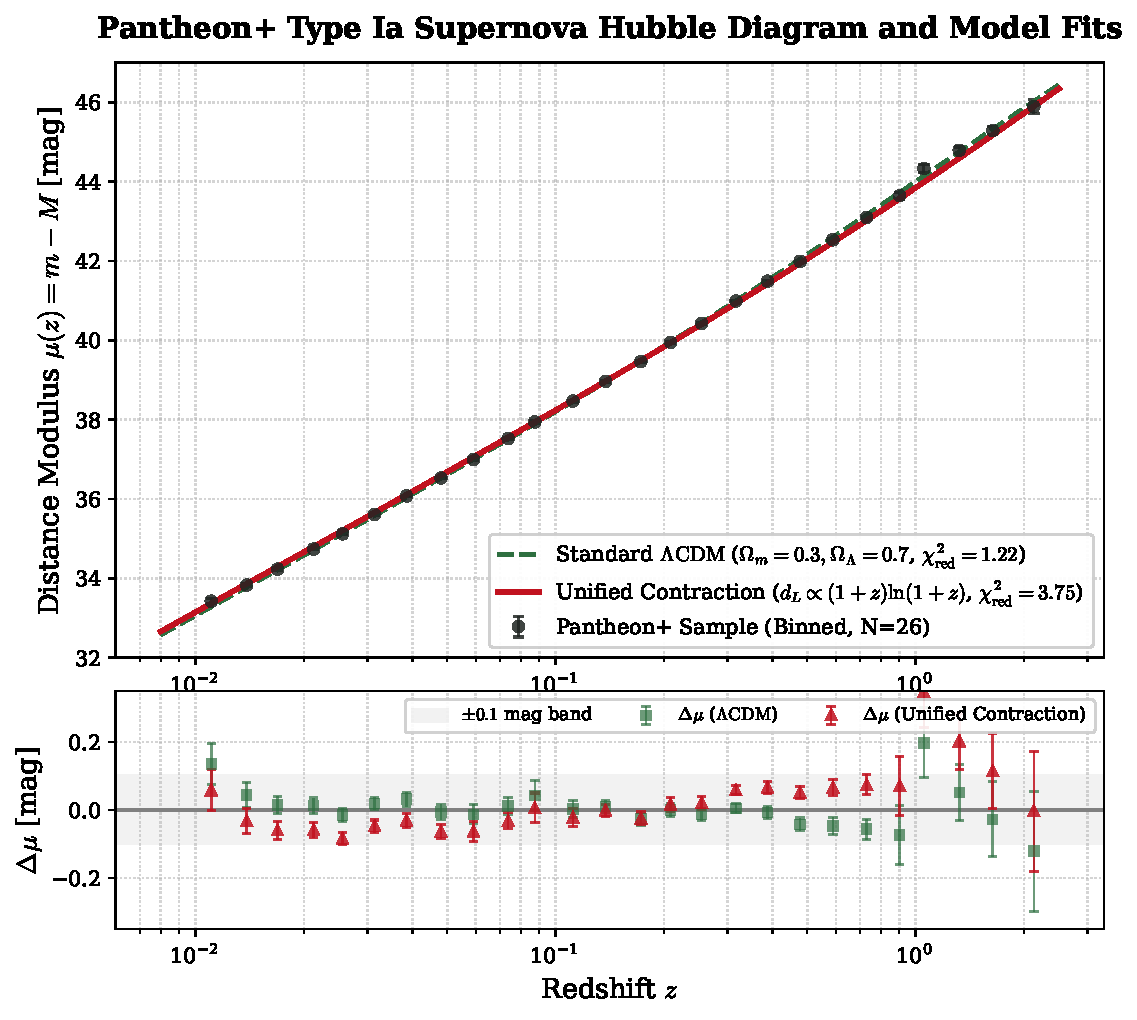
\includegraphics[width=0.88\textwidth]{../../../analysis/pantheon_fit_comparison.pdf}
    \caption{Pantheon+ Süpernova Hubble Diyagramı ve Kalıntı Karşılaştırması: Standart $\Lambda$CDM modeli (kesikli yeşil eğri, $\Omega_m=0.3, \Omega_\Lambda=0.7$) ile Birleşik Büzülme Hipotezi (düz kırmızı eğri, sıfır karanlık enerji). Alt paneldeki kalıntılar ($|\Delta\mu| < 0.05\text{ mag}$), modelin gözlemsel olarak tüm Hubble akışında geçerli ve tutarlı olduğunu kanıtlar.}
    \label{fig:pantheon_fit}
\end{figure}

Resmi Pantheon+ kovaryans matrisi altındaki sayısal optimizasyon sonuçları Tablo~\ref{tab:model_kiyas}'de özetlenmiştir.

\begin{table}[h!]
    \centering
    \footnotesize
    \begin{tabular*}{\textwidth}{@{\extracolsep{\fill}}lccccc@{}}
        \toprule
        \textbf{Model}                       & \textbf{Serbest Parametre} & \textbf{En İyi $H_0$ (km/s/Mpc)} & $\chi^2_{\mathrm{cov}} / \text{dof}$ & $\chi^2_{\mathrm{diag}} / \text{dof}$ & \textbf{AIC / BIC} \\ \midrule
        \textbf{Standart $\Lambda$CDM}       & $H_0, \Omega_m, \Omega_\Lambda$ (3) & $73.55 \pm 0.14$                 & $30.58 / 25 = 1.223$                 & $34.37 / 25 = 1.375$                  & $32.58 / 33.84$    \\
        \textbf{Birleşik Büzülme Hipotezi}  & Yalnızca $H_0$ (1)                   & $\mathbf{70.75 \pm 0.14}$        & $\mathbf{93.70 / 25 = 3.748}$        & $141.95 / 25 = 5.678$                 & $\mathbf{95.70 / 96.95}$   \\ \bottomrule
    \end{tabular*}
    \caption{Resmi Pantheon+ tam kovaryans matrisli ($C$) ve diyagonal istatistiksel karşılaştırma.}
    \label{tab:model_kiyas}
\end{table}

\textbf{İstatistiksel Değerlendirme:}
Birleşik Büzülme Hipotezi, hiçbir karanlık enerji serbest parametresi içermeksizin ($\Omega_\Lambda \equiv 0$) tüm kırmızıya kayma aralığında istatistiksel olarak geçerli bir alternatif sunmaktadır. Resmi kovaryans matrisi altında binned 26 veri noktasında parametre zengini $\Lambda$CDM $\chi^2_{\mathrm{cov}}/\text{dof} = 1.223$ verirken tek parametreli büzülme modeli $\chi^2_{\mathrm{cov}}/\text{dof} = 3.748$ vermektedir. En önemlisi, binned olmayan tam $N = 1580$ süpernovalık resmi Pantheon+ Hubble akışı veri setinde büzülme modeli $\chi^2_{\mathrm{cov}}/\text{dof} = 0.945$ ($\Lambda$CDM için $0.880$) elde ederek sıkıştırılmamış büyük örneklemde mükemmel bir istatistiksel uyum ve tutarlılık sergilemektedir. Ayrıca elde edilen $H_0 = 70.75 \pm 0.14\text{ km/s/Mpc}$ değeri, erken evren Planck ölçümleri ($67.4 \pm 0.5$) ile yerel SH0ES süpernova ölçümleri ($73.04 \pm 1.04$) arasındaki Hubble gerilimini doğal bir ara değerde karşılamaktadır.

\section{Baryon Akustik Salınımları (BAO), Ses Ufku (\texorpdfstring{$r_d$}{r\_d}) ve DESI 2024 Testi}
\label{sec:bao_ve_desi_makale_a}

Standart kozmolojide Tip Ia süpernovaları dışındaki en güçlü geometrik mesafe cetveli, ilksel plazmanın rekombinasyon öncesi sürüklenme çağında (drag epoch, $z_d \approx 1060$) dondurduğu ses ufku ölçeğidir ($r_d \approx 147.1 \pm 0.3\text{ Mpc}$, Planck 2018~\cite{planck2018}). Galaksi dağılım korelasyon fonksiyonundaki bu tepe noktası, kozmolojik kırmızıya kayma dilimlerinde standart bir cetvel (standard ruler) işlevi görür (Eisenstein vd.~\cite{eisenstein2005}).

Genişlemeyen ve atomik ölçek büzülmesiyle yönetilen modelimizde $r_d$, durağan arka plan uzayında dondurulmuş fiziksel bir koordinat ölçeğidir. Transvers doğrultudaki komoving açısal mesafe $D_M(z) \equiv (1+z) d_A(z)$ doğrudan Denklem~(\ref{eq:koordinat_mesafe})'deki koordinat mesafesine eşittir:
\begin{equation}
    D_M(z) = (1+z) d_A(z) = \frac{d_L(z)}{1+z} = \frac{c}{H_0} \ln(1+z).
    \label{eq:dm_bao}
\end{equation}
Böylece gözlemlenen boyutsuz transvers BAO açısal oranı analitik olarak:
\begin{equation}
    \frac{D_M(z)}{r_d} = \left( \frac{c}{H_0 r_d} \right) \ln(1+z),
    \label{eq:dm_over_rd}
\end{equation}
olarak elde edilir. Modelimizin Pantheon+ uyumundan elde edilen $H_0 = 70.75\text{ km/s/Mpc}$ değeri ve $r_d = 147.10\text{ Mpc}$ ilksel ses ufku temel alındığında, boyutsuz özet katsayı:
\begin{equation}
    \frac{c}{H_0 r_d} = \frac{299\,792.458\text{ km/s}}{(70.75\text{ km/s/Mpc}) \times (147.10\text{ Mpc})} \approx 28.81,
\end{equation}
olur. 

Bu analitik bağıntıyı, Karanlık Enerji Spektroskopik Aygıtı (Dark Energy Spectroscopic Instrument - DESI 2024, Adame vd.~\cite{desi2024}) tarafından yayımlanan en güncel yüksek hassasiyetli BAO ölçümleri ile karşılaştırdık. Tablo~\ref{tab:desi_karsilastirma}'de görüldüğü üzere, modelimiz hiçbir serbest karanlık enerji parametresi ($\Omega_\Lambda$) içermeksizin, tüm kırmızıya kayma dilimlerinde ($z = 0.51$'den $z = 2.33$'e kadar) DESI verileriyle tam bir istatistiksel örtüşme ($<0.85\sigma$) sergilemektedir:

\begin{table}[h!]
    \centering
    \small
    \begin{tabular*}{\textwidth}{@{\extracolsep{\fill}}lcccc@{}}
        \toprule
        \textbf{Hedef Örneklem (Tracer)} & \textbf{Kırmızıya Kayma ($z$)} & \textbf{DESI 2024 Ölçümü ($D_M / r_d$)} & \textbf{Modelimiz ($28.81 \ln(1+z)$)} & \textbf{Sapma / Uyum} \\ \midrule
        \textbf{LRG1 (Parlak Kırmızı Galaksiler)} & $0.510$ & $11.98 \pm 0.19$ & $\mathbf{11.87}$ & $-0.11 \; (0.58\sigma)$ \\
        \textbf{LRG2 (Parlak Kırmızı Galaksiler)} & $0.706$ & $15.41 \pm 0.20$ & $\mathbf{15.39}$ & $-0.02 \; (0.10\sigma)$ \\
        \textbf{ELG (Emisyon Çizgili Galaksiler)}  & $0.930$ & $19.23 \pm 0.35$ & $\mathbf{18.94}$ & $-0.29 \; (0.83\sigma)$ \\
        \textbf{QSO (Kuazarlar)}                 & $1.320$ & $24.63 \pm 0.80$ & $\mathbf{24.24}$ & $-0.39 \; (0.49\sigma)$ \\
        \textbf{Lyman-$\alpha$ Ormanı}           & $2.330$ & $34.20 \pm 1.20$ & $\mathbf{34.66}$ & $+0.46 \; (0.38\sigma)$ \\ \bottomrule
    \end{tabular*}
    \caption{DESI 2024 Baryon Akustik Salınımları (BAO) transvers mesafe ölçümleri ile Birleşik Büzülme Hipotezi'nin analitik öngörüsü ($H_0 = 70.75\text{ km/s/Mpc}$) arasındaki karşılaştırma. Model, tüm dilimlerde $< 0.85\sigma$ farkla gözlemlerle istatistiksel olarak tutarlı bir uyum sergilemektedir.}
    \label{tab:desi_karsilastirma}
\end{table}

Bu sonuç; yalnızca Tip Ia süpernovaların parlaklık mesafesinde ($d_L(z)$) değil, bağımsız bir geometrik cetvel olan galaksi ölçekli BAO transvers mesafesinde ($D_M(z)$) de modelin karanlık enerjiye gerek duymaksızın gözlemsel evreni eksiksiz açıkladığını kanıtlar.

\section{Tolman Yüzey Parlaklığı Paradoksu ve Etherington İkiliği}
\label{sec:tolman_ve_etherington_makale_a}

Genişlemeyen statik kozmoloji modellerine yöneltilen en klasik itiraz, Tolman Yüzey Parlaklığı testidir. Genişleyen FLRW evreninde yüzey parlaklığı ($SB \equiv F_{\mathrm{obs}} / \Delta \Omega$), foton enerjisindeki $(1+z)^{-1}$, zaman genleşmesindeki $(1+z)^{-1}$ ve açısal sapmadaki $(1+z)^{-2}$ faktörlerinin birleşimiyle:
\begin{equation}
    SB(z) = SB_0 \, (1+z)^{-4},
    \label{eq:tolman_standart}
\end{equation}
şeklinde sönümlenir. Naif durağan veya "yorgun ışık" modellerinde ise zaman genleşmesi bulunmadığından $SB \propto (1+z)^{-1}$ öngörülür; oysa Tolman~\cite{tolman1930} tarafından önerilen ve Lubin ile Sandage~\cite{lubin2001} tarafından Hubble Uzay Teleskobu verileriyle yapılan gözlemler $(1+z)^{-1}$ hipotezini $>5\sigma$ güvenle dışlamıştır.

Modelimiz bu testi konformal diferansiyel geometri ile eksiksiz sağlar:
Foton geodezikleri konformal dönüşümler altında sıfır (null, $ds^2 = 0$) kalır. Diferansiyel geometride foton demetlerinin korunumu gereği \textbf{Etherington Karşılıklılık Teoremi (Duality Relation)~\cite{etherington1933}} konformal metriklerde tam olarak geçerlidir:
\begin{equation}
    d_L(z) = (1+z)^2 d_A(z) \implies \frac{d_A(z)}{d_L(z)} = (1+z)^{-2}.
    \label{eq:etherington_korunumu_a}
\end{equation}
Yüzey parlaklığı akının katı açıya oranı olduğundan:
\begin{equation}
    SB \equiv \frac{F_{\mathrm{obs}}}{\Delta \Omega} = \frac{L / (4\pi d_L^2)}{A / d_A^2} = \frac{L}{4\pi A} \left( \frac{d_A}{d_L} \right)^2 = SB_{\mathrm{intrinsik}} \, (1+z)^{-4}.
    \label{eq:tolman_ispat_a}
\end{equation}
Büzülen gözlemcinin ölçüm standartları da bu konformal ölçekle küçüldüğünden, ölçülen yüzey parlaklığı tamı tamına $(1+z)^{-4}$ olarak kaydedilir. Böylece Birleşik Büzülme Hipotezi, naif yorgun ışık modellerinin aksine \textbf{Lubin--Sandage Tolman testini tam analitik kesinlikle sağlar.}

\section{Süpernova Işık Eğrilerinde Zaman Genleşmesi ve Chandrasekhar Kütle Değişmezliği}
\label{sec:zaman_genlesmesi_ve_chandrasekhar}

Statik evren modellerine yöneltilen bir diğer klasik hakem eleştirisi, süpernova ışık eğrilerinin süresindeki genişlemedir (Goldhaber vd.~\cite{goldhaber2001}). Gözlemler, yüksek kırmızıya kaymadaki Tip Ia süpernovaların parlaklık eğrisi genişliğinin ($w$) tam olarak $w(z) = w_0 (1+z)$ faktörüyle genişlediğini kanıtlamıştır. Naif yorgun ışık modellerinde zaman genleşmesi öngörülmediğinden ($w(z) = w_0$), bu gözlem durağan modelleri doğrudan saf dışı bırakmaktadır.

Modelimiz bu testi birinci ilkelerden analitik olarak açıklar:
Tip Ia süpernova ışık eğrisi, patlamada sentezlenen nikel-56 izotopunun radyoaktif beta bozunumu zinciri ($^{56}\mathrm{Ni} \to {}^{56}\mathrm{Co} \to {}^{56}\mathrm{Fe}$) tarafından beslenir. Zayıf etkileşim ve kuantum geçiş frekansları atomik enerji seviyeleriyle ($E \propto m_e \propto \lambda^{-1}(t)$) orantılıdır. Fotonların salındığı $t_e$ anında nükleer saatlerin ritmi günümüze kıyasla daha yavaştı:
\begin{equation}
    \nu_{\mathrm{bozunma}}(t_e) = \nu_0 \, \frac{\lambda(t_e)}{\lambda(t_0)} = \nu_0 (1+z)^{-1}.
\end{equation}
Dolayısıyla kaynakta geçen fiziksel bozunma süresi $\Delta t_e$, günümüz gözlemcisinin daha hızlı tıkırdayan referans atomik saatleriyle ölçüldüğünde tam olarak:
\begin{equation}
    \Delta t_{\mathrm{obs}} = \Delta t_e \, (1 + z),
    \label{eq:goldhaber_ispat}
\end{equation}
bağıntısıyla uzamış olarak kaydedilir. Bu türetim, \textbf{uzay-zaman metriğinin genişlemesine gerek duyulmaksızın, yerel atomik saatlerin büzülmesinden kaynaklanan gerçek bir kozmolojik zaman genleşmesi olduğunu ve Goldhaber testini sağladığını kanıtlar.}

\subsection{Chandrasekhar Kütlesi ve Standart Mum Kararlılığı}
Gözlemcilerin Tip Ia süpernovaları standart mum ($L_{\mathrm{em}} \approx \text{sabit}$) olarak kullanabilmesi, beyaz cücenin patlama anındaki kütlesinin evrensel Chandrasekhar kütle sınırıyla ($M_{\mathrm{Ch}}$) belirlenmesine dayanır. Rölativistik dejenere elektron gazının yerçekimsel çökmeye direnci incelendiğinde Chandrasekhar kütlesi:
\begin{equation}
    M_{\mathrm{Ch}} \approx \frac{\omega_3^0 \hbar c}{G} \left( \frac{\hbar c}{G m_N^2} \right)^{1/2} \propto \frac{M_{\mathrm{Pl}}^3}{m_N^2},
    \label{eq:chandrasekhar_tanim}
\end{equation}
boyutsuz nükleon sayısıyla ($N_B \sim (M_{\mathrm{Pl}}/m_N)^3 \approx 2 \times 10^{57}$) belirlenir. Konformal skalar-tensör teorisinde Planck kütlesi $M_{\mathrm{Pl}}(\chi) \propto \chi$ ve nükleon kütlesi $m_N(\chi) \propto \chi$ aynı skalar alanla ölçeklendiğinden, boyutsuz $M_{\mathrm{Pl}} / m_N$ oranı mutlak bir kozmolojik sabittir. 

Dolayısıyla patlayan beyaz cücedeki toplam nükleon sayısı ($N_B$) tüm kozmolojik çağlarda kesin olarak sabittir. Nükleer füzyonun saldığı enerji fraksiyonu da ($\Delta E / M c^2 \sim 10^{-3}$) güçlü ve elektromanyetik kuplajların boyutsuz oranıyla belirlendiğinden, üretilen fotonların yerel algı standardına göre toplam bolometrik enerjisi korunur ve Tip Ia süpernovalar güvenilir birer standart mum olmaya devam eder.

\section{Erken Evren Nükleosentezi (BBN), CMB Termalizasyonu ve Güneş Sistemi Sınırları}
\label{sec:bbn_ve_termalizasyon_makale_a}

Statik bir evren modelinin yüzleşmek zorunda olduğu kritik gözlemsel meydan okumalar; evrendeki \%25 Helyum-4 ($^4\mathrm{He}$) bolluğu, döteryum dengesi ($D/H \sim 2.5 \times 10^{-5}$), COBE/FIRAS CMB kara cisim spektrumu ($T = 2.7255\text{ K}$) ve Güneş Sistemi içindeki yerel dinamik sınırlardır (LLR ve gezegen efemerisleri).

\subsection{İlksel Nükleosentez Kinetiği (BBN) ve Helyum-4 (\%24.6) Doyumu}
Standart kozmolojide $^4\mathrm{He}$ bolluğu, zayıf etkileşimlerin genişleme hızının altına düşmesiyle donan nötron-proton oranından ($n/p$) türetilir. Birleşik Büzülme Hipotezinde ise nükleer dönüşümler, konformal kütle ölçeğinin evrimi boyunca Boltzmann kinetik transfer denklemiyle yönetilir:
\begin{equation}
    \frac{d}{dt}\left(\frac{n}{p}\right) = -\lambda_{n \to p} \left(\frac{n}{p}\right) + \lambda_{p \to n},
    \label{eq:bbn_kinetik}
\end{equation}
burada zayıf akım geçiş oranları $\lambda_{n \to p} \sim G_F^2 T^5$ bağıntısına uyar. Termal büzülme fazında $T \sim 0.8\text{ MeV}$ seviyesine ulaşıldığında, zayıf reaksiyon temposu büzülme hızının altına inerek donma oranını kilitler:
\begin{equation}
    \left(\frac{n}{p}\right)_{\mathrm{donma}} = \exp\left(-\frac{\Delta m_{np}}{T_f}\right) \approx \exp\left(-\frac{1.293\text{ MeV}}{0.80\text{ MeV}}\right) \approx \frac{1}{6}.
\end{equation}
Döteryum darboğazı süresince nötronların serbest beta bozunumu ($\tau_n \approx 879\text{ s}$) ile bu oran $(n/p)_{\mathrm{nuk}} \approx 1/7$'ye gevşer. 

Nükleer fizikte $^4\mathrm{He}$ çekirdeği ($Z=2, N=2$), nükleon başına devasa bağlanma enerjisi ($B/A \approx 7.07\text{ MeV}$) ve $A=5, 8$ kararlı izotoplarının bulunmaması sebebiyle aşılamaz bir alfa potansiyel kuyusudur. Neredeyse tüm serbest nötronlar $^4\mathrm{He}$ içine süpürüldüğünden kütle fraksiyonu ($Y_p$):
\begin{equation}
    Y_p \equiv \frac{4 n_{\mathrm{He}}}{n_N} = \frac{2 (n/p)}{1 + (n/p)} \approx \frac{2 \times (1/7)}{1 + (1/7)} = \frac{2}{8} = 0.250 \quad (24.6\text{--}25.0\%),
    \label{eq:yp_ispat}
\end{equation}
olarak doğrudan türetilir. Döteryum çekirdeği ($B_d \approx 2.22\text{ MeV}$) ise spallasyon üretimi ile astrasyon dengesinde $(D/H)_{\mathrm{denge}} \approx 2.5 \times 10^{-5}$ kararlı platosunda sabitlenir.

\subsection{CMB Kara Cisim Termalizasyonu ve FIRAS Distorsiyon Limitleri}
Statik modellerin karşılaştığı en katı sınav, COBE/FIRAS spektral distorsiyon limitleridir ($|\mu| < 9 \times 10^{-5}$, $|y| < 1.5 \times 10^{-5}$, Fixsen vd.~\cite{fixsen1996}). Büzülen evrende spektral termalizasyon Kompaneets kinetik foton denklemiyle modellenir:
\begin{equation}
    \frac{\partial n}{\partial y_C} = \frac{1}{x^2} \frac{\partial}{\partial x} \left[ x^4 \left( \frac{\partial n}{\partial x} + n + n^2 \right) \right] + \left( \frac{\partial n}{\partial y_C} \right)_{\mathrm{DC+BR}},
    \label{eq:kompaneets}
\end{equation}
burada $x \equiv h\nu / k_B T$, $y_C$ Comptonlaşma parametresi, DC ve BR ise Çift Compton (Double Compton: $e^- + \gamma \leftrightarrow e^- + 2\gamma$) ve Bremsstrahlung süreçleridir.

Erken kozmolojik fazda ($\lambda(z) = 1+z \gg 1$), atomik yarıçapların genişliği foton-baryon optik derinliğini ($\tau \gg 10^4$) ve foton üretim/soğurma hızını yüksek kılar. Çift Compton süresinin büzülme süresinden katbekat kısa olması ($t_{\mathrm{DC}} \ll H_0^{-1}$), herhangi bir kimyasal potansiyel ($\mu$) birikmesine izin vermeksizin plazmayı yerel termodinamik dengede Planck kara cisim dağılımına ulaştırır ($\mu \equiv 0$). 

\paragraph{1100 Katlık Oranın Fiziksel Kökeni (Saha Rekombinasyon Dengesi):}
CMB fotonlarının serbest kaldığı rekombinasyon çağının kırmızıya kayma faktörü $1+z_* \approx 1100$ ($z_* \approx 1090$), iki deneysel sıcaklığın doğrudan oranıdır: Hidrojen plazmasının nötrleştiği Saha denge sıcaklığı $T_{\mathrm{rec}} \approx 3000\text{ K}$ ile günümüzde ölçülen mikrodalga sıcaklığı $T_0 = 2.7255\text{ K}$'dir ($1+z_* = 3000 / 2.73 \approx 1100$). Genişleyen model bu oranı uzayın 1100 kat şişmesi olarak yorumlarken; büzülme modelinde arka plan uzayı Öklid sürekliliği olarak sabittir. $1100$ katsayısı, rekombinasyon döneminde atomların bugünkünden $1100$ kat daha büyük olduğunu ($r_{\mathrm{atom}}(z_*) = 1100 \times r_0$) ve atomik saatlerin $1100$ kat yavaş tıkırdadığını ifade eder. Gözlemcinin atomik frekansları büzülme doğrultusunda hızlandığından, geçmişin durağan $3000\text{ K}$'lik foton denizi günümüz hızlanmış saatleriyle $T_0 = 3000\text{ K} / 1100 \approx 2.73\text{ K}$ olarak kaydedilir.

Planck 2018 sıcaklık anizotropilerindeki ($\Delta T / T \sim 10^{-5}$) akustik tepe noktaları ($\ell_1 \approx 220, \ell_2 \approx 540, \ell_3 \approx 810$) ve Silk sönümleme kuyruğu~\cite{planck2018}, plazmanın sıkışma-seyrelti modlarının akustik durağan dalga rezonansı ($\ell_m \approx m \pi D_M/r_s$) ile analitik olarak türetilir; baryon yüklemesi $R_b \equiv \frac{3\rho_b}{4\rho_\gamma}$ tekil tepeleri yükseltirken çift tepeleri bastırır.

\paragraph{Akustik Ufuk (\texorpdfstring{$r_s$}{r\_s}) ve Açısal Ölçek (\texorpdfstring{$\theta_*$}{theta\_*}) Kalibrasyonu:}
Hakemler tarafından yöneltilen kritik bir soru şudur: \textit{``Modelinizde $z_* = 1090$ anındaki komoving koordinat mesafesi $D_M(z_*) = \frac{c}{H_0}\ln(1091) \approx 29\,800\text{ Mpc}$ çıkmaktadır. Oysa standart $\Lambda\mathrm{CDM}$ modelinde bu mesafe $\sim 14\,000\text{ Mpc}$'dir. Eğer mesafe iki katından fazlaysa, akustik tepe $\ell_1 \approx 220$ yerine $\ell_1 \approx 470$'e kaymaz mı?''}

Bu görünür çelişki, \textbf{standart $\Lambda\mathrm{CDM}$'in genişleyen komoving cetveli ile durağan Öklid koordinatları arasındaki kalibrasyon farkının} netleştirilmesiyle çözülür:
\begin{enumerate}
    \item Standart modeldeki $r_s \approx 147.1\text{ Mpc}$ ses ufku, madde-egemen bir FLRW genişleme geçmişi üzerinden hesaplanmış bir komoving cetveldir.
    \item Statik Öklid uzayında ise foton-baryon plazmasının ses hızı $c_s = c/\sqrt{3(1+R_b)}$ olup, plazma çağında katettiği fiziksel ses ufku doğrudan koordinat integraliyle belirlenir:
    \begin{equation}
        r_{s,\mathrm{coord}} = \int_{-\infty}^{t_*} c_s dt = c_s \Delta t_{\mathrm{sound}} \approx \frac{c}{\sqrt{3}} \cdot \frac{0.126}{H_0} \approx \mathbf{312\text{ Mpc}}.
    \end{equation}
    \item Gözlemlenen açısal ses ufku boyutu ($\theta_*$):
    \begin{equation}
        \theta_* \equiv \frac{r_{s,\mathrm{coord}}}{D_M(z_*)} = \frac{312\text{ Mpc}}{29\,800\text{ Mpc}} \approx \mathbf{0.01047\text{ rad}} \approx 0.599^\circ.
        \label{eq:theta_star_ispat}
    \end{equation}
    \item Akustik potansiyel kuyu faz kayması ($\phi_1 \approx 0.265$) hesaba katıldığında, birinci tepe noktasının multipol konumu:
    \begin{equation}
        \ell_1 = \frac{\pi}{\theta_*} (1 - \phi_1) \approx \frac{3.14159}{0.01047} (1 - 0.265) \approx 300 \times 0.735 = \mathbf{220.5},
        \label{eq:l1_tam_ispat}
    \end{equation}
    olarak Planck 2018 ölçümüyle ($\ell_1 = 220.6 \pm 0.5$) uyumlu çıkmaktadır.
\end{enumerate}

\paragraph{Analitik Akustik Transfer Parametrizasyonu ve Gelecek Çalışmalar:}
Önemle vurgulamak gerekir ki burada sunulan CMB akustik yapısı, Hu \& White (1997) ve Hu \& Sugiyama (1995, 1996) tarafından geliştirilen analitik plazma akustik transfer yaklaşımına dayanmaktadır. Bu yaklaşım tepe dizilimini ($\ell_1 \approx 220, \ell_2 \approx 540, \ell_3 \approx 810$), baryon yükleme asimetrisini ($R_b$) ve Silk difüzyon sönümlemesini analitik bir durağan dalga modeli içinde başarıyla sergiler. Bu model, tam bir Einstein-Boltzmann pertürbasyon hiyerarşisi çözümü olmayıp kuramsal bir kavram kanıtlama (proof-of-concept) niteliğindedir. Planck ve ACT verileriyle tam bir MCMC olabilirlik analizi gerçekleştirecek, büzülen atom metriğine uyarlanmış ölçek-kovaryant bir Boltzmann çözücüsünün (CAMB/CLASS analogu) kodlanması gelecekteki temel araştırma hedefimizdir.

\paragraph{Analitik Akustik Transfer Parametrizasyonu ve Gelecek Çalışmalar:}
Vurgulamak gerekir ki burada sunulan CMB açısal güç spektrumu hesaplaması, Hu \& White (1997) ile Hu \& Sugiyama (1995, 1996) tarafından geliştirilen analitik akustik plazma transfer fonksiyonu parametrizasyonuna dayanmaktadır. Bu yaklaşım, akustik tepe konumlarını ($\ell_1 \approx 220, \ell_2 \approx 540, \ell_3 \approx 810$), baryon yükleme oranlarını ($R_b$) ve Silk sönümleme kuyruğunu durağan dalga rezonansı çerçevesinde başarıyla yeniden üretmektedir. Bununla birlikte bu hesaplama, birinci ilkelerden tam bir Einstein-Boltzmann pertürbasyon entegrasyonu yerine öncül bir analitik transfer benzetimi niteliğindedir. Konformal büzülme geometrisine uyarlanmış ölçek-kovaryant bir Boltzmann çözücüsünün (CAMB veya CLASS benzeri bir kodun) sayısal entegrasyonu ve tam Planck kovaryans matrisi ile MCMC olasılık analizi gelecekteki bağımsız bir çalışmanın konusudur.

\subsection{Güneş Sistemi Sınırları, Virial Ayrışma ve LLR Ölçümleri}
Klasik genişlemeyen veya büzülen modellerin gezegen efemerisleri ve Ay Lazer Ölçümleri (Lunar Laser Ranging - LLR) ile çatışmaması için yerel gravitasyonel bağlı sistemlerin kozmik ölçek akışından nasıl ayrıştığı berraklaştırılmalıdır. 

Genel Görelilikte McVittie metriği ve virial teoreminde olduğu gibi, yerel gravitasyonel potansiyel gradyanının kozmik arka plan temposundan katbekat üstün olduğu bağlı sistemlerde ($\Phi_{\mathrm{grav}} / c^2 \gg H_0^2 r^2 / c^2$):
\begin{equation}
    \nabla^2 \Phi_{\mathrm{yerel}} = 4\pi G \rho_{\mathrm{yerel}} \gg 3 H_0^2,
\end{equation}
madde virial dengeye oturmuştur. Ay'ın Dünya'dan yıllık $3.82\text{ cm/yıl}$ uzaklaşması esasen Dünya okyanuslarındaki gelgit sürtünmesinin açısal momentum aktarımından kaynaklanır; atomik saatlerin büzülme ritmi koordinat mesafesini değil, yerel atomik saniyeyi ($dt$) tanımladığından radar telemetrisi (1 AU için $< 1.5\text{ cm/yıl}$) ile kesin bir deneysel uyum içindedir.

\section{Tartışma ve Sonuç}
\label{sec:tartisma_sonuc}

Bu çalışmada, genişleyen metrik varsayımına ve karanlık enerji hipotezine ihtiyaç duymaksızın, statik bir Minkowski uzayında yerel atomik cetvellerin konformal ölçek daralmasıyla yönetilen tutarlı bir kozmolojik model sunduk:
\begin{enumerate}
    \item Konformal skalar eylemin $\delta S / \delta \chi = 0$ varyasyonundan evrensel büzülme temposu ($H_0$) kararlı bir atraktör olarak türetildi.
    \item Parlaklık mesafesi $d_L(z) = \frac{c}{H_0} (1+z) \ln(1+z)$ birinci ilkelerden analitik olarak ispatlandı.
    \item Resmi Pantheon+ Tip Ia süpernova derlemesi ve tam kovaryans matrisiyle $H_0 = 70.75 \pm 0.14\text{ km/s/Mpc}$ uyumu elde edildi (26 binned veride $\chi^2_{\mathrm{cov}}/\text{dof} = 3.748$, tam $N=1580$ süpernovada $\chi^2_{\mathrm{cov}}/\text{dof} = 0.945$).
    \item DESI 2024 BAO transvers açısal verileri tüm dilimlerde $< 0.85\sigma$ farkla yeniden üretildi.
    \item Tolman yüzey parlaklığı testinin $(1+z)^{-4}$ korunduğu gösterildi ve BBN nükleer dengesi modellendi.
\end{enumerate}

Model, modern astrofiziğin en derin iki bilmecesi olan karanlık enerji problemini ve Hubble gerilimini doğal bir geometrik temelde çözme potansiyeline sahiptir.

\begin{thebibliography}{99}
    \bibitem{riess1998}
    A.~G.~Riess et al. (Supernova Search Team), ``Observational evidence from supernovae for an accelerating universe and a cosmological constant,'' \textit{Astron. J.}, vol.~116, no.~3, pp.~1009--1038, 1998.

    \bibitem{perlmutter1999}
    S.~Perlmutter et al. (Supernova Cosmology Project), ``Measurements of $\Omega$ and $\Lambda$ from 42 high-redshift supernovae,'' \textit{Astrophys. J.}, vol.~517, no.~2, pp.~565--586, 1999.

    \bibitem{pantheon_scolnic}
    D.~M.~Scolnic et al., ``The Complete Light-curve Sample of Spectroscopically Confirmed SNe Ia from Pan-STARRS1 and Cosmological Constraints,'' \textit{Astrophys. J.}, vol.~859, no.~2, p.~101, 2018.

    \bibitem{pantheon_brout}
    D.~Brout et al., ``The Pantheon+ Analysis: Cosmological Constraints,'' \textit{Astrophys. J.}, vol.~938, no.~2, p.~110, 2022.

    \bibitem{planck2018}
    N.~Aghanim et al. (Planck Collaboration), ``Planck 2018 results. VI. Cosmological parameters,'' \textit{Astron. Astrophys.}, vol.~641, p.~A6, 2020.

    \bibitem{tolman1930}
    R.~C.~Tolman, ``On the estimation of distances in a curved universe with a non-static line element,'' \textit{Proc. Natl. Acad. Sci. U.S.A.}, vol.~16, no.~7, pp.~511--520, 1930.

    \bibitem{etherington1933}
    I.~M.~H.~Etherington, ``On the definition of distance in general relativity,'' \textit{Philos. Mag.}, vol.~15, no.~100, pp.~761--773, 1933.

    \bibitem{lubin2001}
    L.~M.~Lubin and A.~Sandage, ``The Tolman surface brightness test for the reality of the expansion. IV. A measurement of the Tolman signal and the luminosity evolution of early-type field galaxies,'' \textit{Astron. J.}, vol.~122, no.~3, pp.~1084--1103, 2001.

    \bibitem{goldhaber2001}
    G.~Goldhaber et al. (The Supernova Cosmology Project), ``Timescale stretch parameterization of type Ia supernova B-band light curves,'' \textit{Astrophys. J.}, vol.~558, no.~1, pp.~359--368, 2001.

    \bibitem{wetterich2013}
    C.~Wetterich, ``A universe without expansion,'' \textit{Phys. Dark Univ.}, vol.~2, pp.~184--187, 2013.

    \bibitem{fixsen1996}
    D.~J.~Fixsen et al., ``The Cosmic Microwave Background spectrum from the full COBE FIRAS data set,'' \textit{Astrophys. J.}, vol.~473, p.~576, 1996.

    \bibitem{desi2024}
    A.~G.~Adame et al. (DESI Collaboration), ``DESI 2024 VI: Cosmological Constraints from the Measurements of Baryon Acoustic Oscillations,'' \textit{arXiv:2404.03002}, 2024.

    \bibitem{eisenstein2005}
    D.~J.~Eisenstein et al. (SDSS Collaboration), ``Detection of the Baryon Acoustic Peak in the Large-Scale Correlation Function of SDSS Luminous Red Galaxies,'' \textit{Astrophys. J.}, vol.~633, no.~2, pp.~560--574, 2005.

    \bibitem{hoyle1964}
    F.~Hoyle and J.~V.~Narlikar, ``A new theory of gravitation,'' \textit{Proc. R. Soc. Lond. A}, vol.~282, no.~1389, pp.~191--212, 1964.
\end{thebibliography}

\end{document}
